\documentclass[12pt]{examdesign}
\usepackage[spanish]{babel}
\OneKey
\usepackage[utf8]{inputenc}
\usepackage[T1]{fontenc}
\usepackage{amsmath}
\usepackage{pifont}
%-----------------------------------------------------------------------------------------------
%\usepackage{gfsartemisia-euler}
\usepackage{graphicx}
\usepackage{float}
\usepackage{amscd}
\usepackage{amsfonts}
\usepackage{amssymb}
\usepackage{mathtools}
\usepackage{amsthm}
\usepackage[all]{xy}
\usepackage{enumitem}
\usepackage{multicol}
\usepackage{verbatim}
\usepackage[colorlinks=true,
breaklinks=true,
linkcolor=blue,
urlcolor=red,
bookmarksopen=true]{hyperref}
\usepackage[pdftex,dvipsnames]{xcolor}
\definecolor{aqua}{rgb}{0.0, 1.0, 1.0}
\definecolor{caribbeangreen}{rgb}{0.0, 0.8, 0.6}
\definecolor{tealgreen}{rgb}{0.0, 0.51, 0.5}
\definecolor{upforestgreen}{rgb}{0.0, 0.27, 0.13}
\definecolor{napiergreen}{rgb}{0.16, 0.5, 0.0}
\definecolor{capri}{rgb}{0.0, 0.75, 1.0}
\definecolor{calpolypomonagreen}{rgb}{0.12, 0.3, 0.17}
\definecolor{azure(colorwheel)}{rgb}{0.0, 0.5, 1.0}
\definecolor{dukeblue}{rgb}{0.0, 0.0, 0.61}
\definecolor{bole}{rgb}{0.47, 0.27, 0.23}
\definecolor{gris}{gray}{0.975}
%----------------------------------------------------------------------------------------------
% Si desea utilizar \@@line para definir su propio encabezado de examen o palabras del encabezado, 
% asegúrese de usar \makeatletter y \makeatother en los lugares apropiados, de lo contrario 
% podría obtener errores.
%-----------------------------------------------------------------------------------------------
\theoremstyle{plain}
\newtheorem{theorem}{Theorem}[section]
\newtheorem{thm}[theorem]{Teorema}
\newtheorem{cor}[theorem]{Corolario}
\newtheorem{lem}[theorem]{Lema}
\newtheorem{pro}[theorem]{Proposición}
\newtheorem{axs}[theorem]{Axiomas}
\newtheorem{axi}[theorem]{Axioma}
\theoremstyle{definition}
\newtheorem{exas}[theorem]{Ejemplos}
\newtheorem{exa}[theorem]{Ejemplo}
\newtheorem{defi}[theorem]{Definición}
\theoremstyle{remark}
\newtheorem{rmk}[theorem]{Observación}
\newtheorem{step}{Step}
\newtheorem{xca}[theorem]{Ejercicio}
\newtheorem{prob}[theorem]{Pregunta}
\newtheorem{rmks}[theorem]{Observaciones}
\newtheorem*{proofmt}{Prueba del Teorema Principal}
\usepackage[centerlast,small,sc]{caption}
\setlength{\captionmargin}{20pt}
\newcommand{\axref}[1]{Axioma~\ref{#1}}
\newcommand{\defref}[1]{\textbf{Definición}~\ref{#1}}
\newcommand{\coref}[1]{\textbf{Corolario}~\ref{#1}}
\newcommand{\thref}[1]{\textbf{Teorema}~\ref{#1}}
\newcommand{\lref}[1]{\textbf{Lema}~\ref{#1}}
\newcommand{\exaref}[1]{Ejemplo~\ref{#1}}
\newcommand{\xcaref}[1]{Ejercicio~\ref{#1}}
\newcommand{\rmkref}[1]{Observación~\ref{#1}}
\newcommand{\pref}[1]{\textbf{Proposición}~\ref{#1}}
\newcommand{\fref}[1]{Figura~\ref{#1}}
\newcommand{\tref}[1]{Tabla~\ref{#1}}
\newcommand{\cref}[1]{\textbf{Capítulo}~\ref{#1}}
\newcommand{\sref}[1]{\textbf{Sección}~\ref{#1}}
\newcommand{\aref}[1]{Apéndice~\ref{#1}}
\newcommand{\eref}[1]{Ecuación~\eqref{#1}}
\newcommand{\dref}[1]{Diagrama~\eqref{#1}}
\usepackage{makeidx}
\usepackage{tikz,tkz-tab}%
\usetikzlibrary{matrix,arrows,positioning,shadows,shadings,backgrounds,
	calc, shapes, tikzmark}
\usepackage{tcolorbox, empheq}%
\tcbuselibrary{skins,breakable,listings,theorems}

\tcbset{opteqC/.style={skin=beamer,colback=red!1!white}}
\newcommand{\celda}[2]{
	\begin{minipage}{#1mm}
		\centering
		\vspace{2mm}
		#2
		\vspace{2mm}
	\end{minipage}
}
\makeatletter
\begin{examtop}
	\@@line{\parbox{3in}{\classdata \\[0.5cm]
			\textcolor{upforestgreen}{\textbf{\underline{T.P.N$^\circ$}}~\fbox{\textsc{7}}} \examtype}
		%                  ^^^^^^
		\hfill
		\parbox{3in}{\normalsize \namedata}}
	\bigskip
\end{examtop}

\def\namedata{\textcolor{upforestgreen}{\textbf{Estudiante}}:\hrulefill \\[\namedata@vspace]
	\textcolor{upforestgreen}{\textbf{Curso y División}}: 1er año, I \\[\namedata@vspace]
	\textcolor{upforestgreen}{\textbf{Profesor}}: Ferreira, Juan David \\[\namedata@vspace]
	\textcolor{upforestgreen}{\textbf{Fecha de Entrega}}:\hrulefill 
}
% manual page 11        
\begin{keytop}%
	\@@line{\hfill \Huge\texttt{\textcolor{upforestgreen}{Respuestas 
				Trabajo Práctico N$^\circ$~\fbox{\textsc{7}}}} \hfill}
	\bigskip
\end{keytop}%
\makeatother
\examname{\textcolor{upforestgreen}{\underline{\textbf{Suma de Fracciones.}}}}

\SectionPrefix{\textcolor{upforestgreen}{\textbf{Sección \arabic{sectionindex}}.} \space}
\Fullpages
\ContinuousNumbering
\DefineAnswerWrapper{}{}
\NumberOfVersions{1}
\class{{\textcolor{upforestgreen}{\large\textbf{E.P.E.S. Nro 51 ``J. G. A.''}}\\[0.5cm]
		\textcolor{upforestgreen}{{\large \textbf{Matemática}}}}}

\begin{document}
	
	
	%-------------------------------             FILLIN       ------------------------%
	\begin{fillin}[title={Completamos los espacios vacíos:}, resetcounter=no]
		
		Recordando que un cálculo mental es aquel que no se escribe en una forma de resolver, donde utilizamos gráficos,
		cálculos auxiliares u otras herramientas que servirán para dar una resolución al problema, resolvemos lo siguiente...
		\begin{question}
			Completamos los espacios vacíos:
			\begin{enumerate}
				\item $\frac{3}{4}+$ \blank{ $\frac{2}{4}$ } =$\frac{5}{4}$.
				\item $\frac{3}{4}+$ \blank{ $\frac{5}{4}$ } =$\frac{8}{4}$.
				\item $\frac{3}{4}+$ \blank{ $\frac{9}{4}$ } =$\frac{12}{4}$.
				\item $\frac{5}{7}+$ \blank{ $\frac{4}{7}$ } =$\frac{9}{7}$.
				\item $\frac{13}{4}-$ \blank{ $\frac{3}{4}$ } =$\frac{10}{4}$.
				\item $\frac{15}{6}-$ \blank{ $\frac{5}{6}$ } =$\frac{10}{6}$.
				\item $\frac{21}{7}-$ \blank{ $\frac{9}{7}$ } =$\frac{12}{7}$.
				\item $\frac{15}{7}-$ \blank{ $\frac{4}{7}$ } =$\frac{11}{7}$.
			\end{enumerate}
        \end{question}
        
        \begin{question}
        	Recordando que una fracción equivalente amplificada de 3 puede ser la siguiente:
        	\begin{equation*}
        		3=\frac{3}{1}=\frac{6}{2}=\frac{9}{3}=\frac{12}{4}=\frac{15}{5}=\frac{18}{6}=\cdots
        	\end{equation*}
        	Esto se utiliza para sumar fracciones, como por ejemplo:
        	\begin{align*}
        	    3+\frac{1}{2}&=\textcolor{red}{\frac{6}{2}}+\frac{1}{2}=\frac{7}{2}&;&&3+\frac{4}{3}&=\textcolor{red}{\frac{9}{3}}+\frac{4}{3}=\frac{13}{3}\\[0.2cm]
        	    3+\frac{1}{4}&=\textcolor{red}{\frac{12}{4}}+\frac{1}{4}=\frac{13}{4}&;&&3+\frac{3}{5}&=\textcolor{red}{\frac{15}{5}}+\frac{3}{5}=\frac{18}{3}
            \end{align*}
        	Escribir estos números como una sola fracción:
        	\begin{enumerate}
        		\item $2+\frac{1}{2}=$ \blank{ $\frac{5}{2}$ }.
        		\item $5+\frac{3}{4}=$ \blank{ $\frac{23}{4}$ }.
        		\item $6+\frac{4}{4}=$ \blank{ $\frac{28}{4}$ }.
        		\item $3+\frac{6}{4}=$ \blank{ $\frac{18}{4}$ }.
        		\item $10+\frac{2}{8}=$ \blank{ $\frac{82}{8}$ }.
        		\item $8+\frac{8}{8}=$ \blank{ $\frac{72}{8}$ }.
        	\end{enumerate}
        \end{question}
	\end{fillin}
	%--------------------------------------------------------------------------------------------%
	\begin{endmatter}
		\centerline{\huge \textcolor{upforestgreen}{\textbf{Suma de Fracciones de igual Denominador:}}}
		\vspace{.4cm}
		\begin{figure}[H]
			\centering
			%\raggedright
			\begin{tikzpicture}
			    \node at (0, 0) {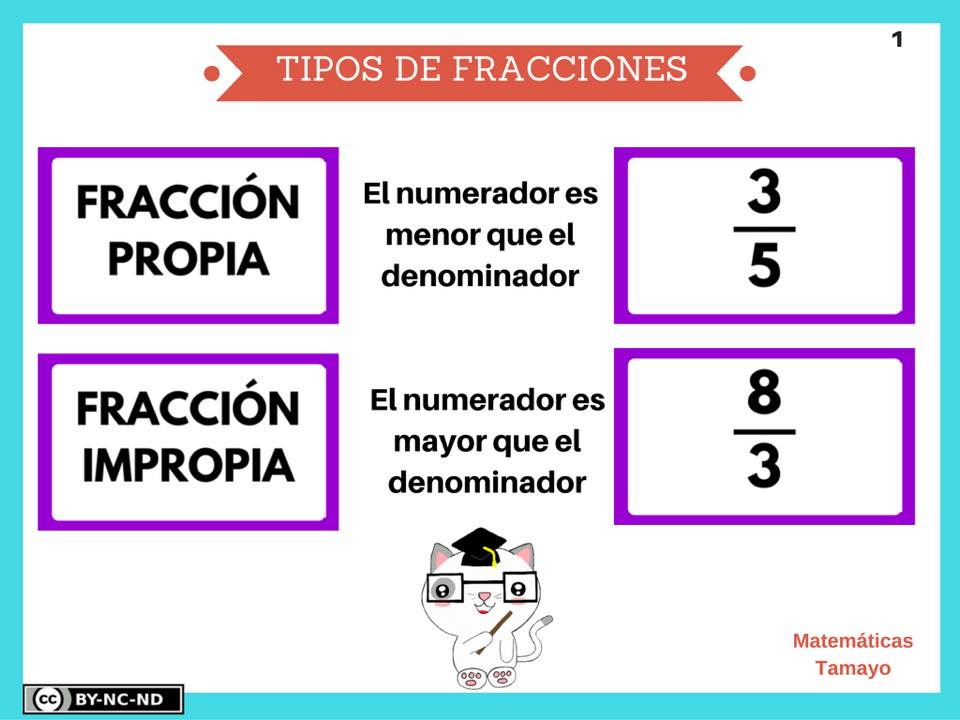
\includegraphics[height=5cm, width=8cm]{fracciones1.jpg}};
			    \node at (8, 0) {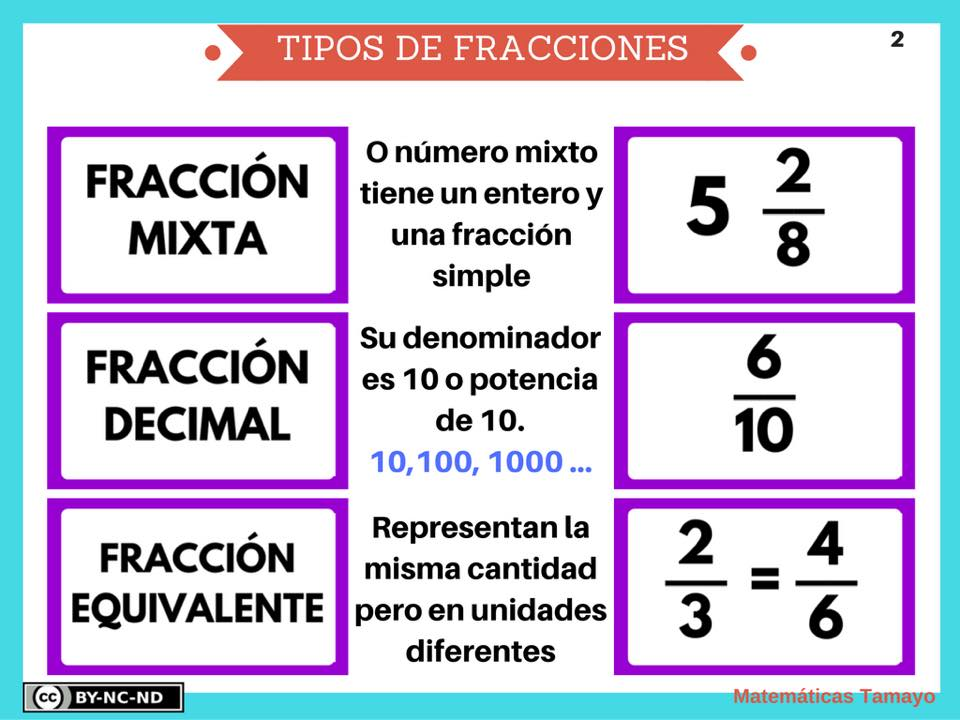
\includegraphics[height=5cm, width=8cm]{fracciones2.jpg}};
			\end{tikzpicture}
		\end{figure}
				
		Supongamos que tenemos la siguiente situación problemática:
		\vspace{.4cm}
		\begin{tcolorbox}[colback=red!10!white, colframe=tealgreen, title=\textit{Para pensar}:]
			\def\blank#1{$\underline{\mbox{\hphantom{#1}}}$}
			\begin{enumerate}%
				\item Pensar con el compañero de al lado hallar la forma correcta completar la oración y justifiquen su respuesta
				\begin{center}
					``\textit{Supongammos que tengo la fracción $\frac{1}{6}$ y le sumamos $\frac{3}{6}$. Entonces, se tiene un total de \blank{$\frac{1}{6} + \frac{3}{6}= \frac{4}{6}$}}''.
				\end{center}
			\end{enumerate}%
			%$\bullet$
		\end{tcolorbox}
	 \textbf{Preguntas a responder:} 
	 \begin{itemize}
	 	\item \textit{¿Qué  vemos que en común $\frac{1}{6}$ y  $\frac{3}{6}$?}
	 	Observemos que cada una de las fracciones poseen el numero $\textcolor{red}{6}$ como \textbf{denominador}.
	 	\item \textit{¿Qué operación matemático involucra resolver esta situación problemática?.}
	 	Resolver dicha situación  problemática que involucra \textbf{la suma de  fracciones de igual denominador denominador}.
	 	\item \textit{¿Cómo pordemos sumar esás fracciones?.} El hecho de que ambas fracciones tengan igual denominador, quiere decir que si a $\frac{1}{6}$ le sumamos $\frac{3}{6}$ se tiene un total de $\frac{1}{\textcolor{red}{6}} + \frac{3}{\textcolor{red}{6}}= \frac{4}{\textcolor{red}{6}}$ y, con esta operación, podemos completar el espacio en blanco.
	 	\item \textit{¿Por  qué  decimos  que  a $\frac{1}{6}$ le sumamos $\frac{3}{6}$ y tenemos como resultado $\frac{4}{6}$}?. Esta respuesta la podemos ver de mejor manera en una explicación más gráfica:
	 	
	 	\begin{figure}[H]
	 		\centering
	 		%\raggedright
	 		\begin{tikzpicture}
	 		\draw[gris, fill = gris] (0,0) rectangle (15, 5);
	 		\draw[ultra thick, caribbeangreen] (0,0) -- (15, 0) -- (15,5) -- (0, 5)-- (0,0);
	 		\node at (4, 2.5) {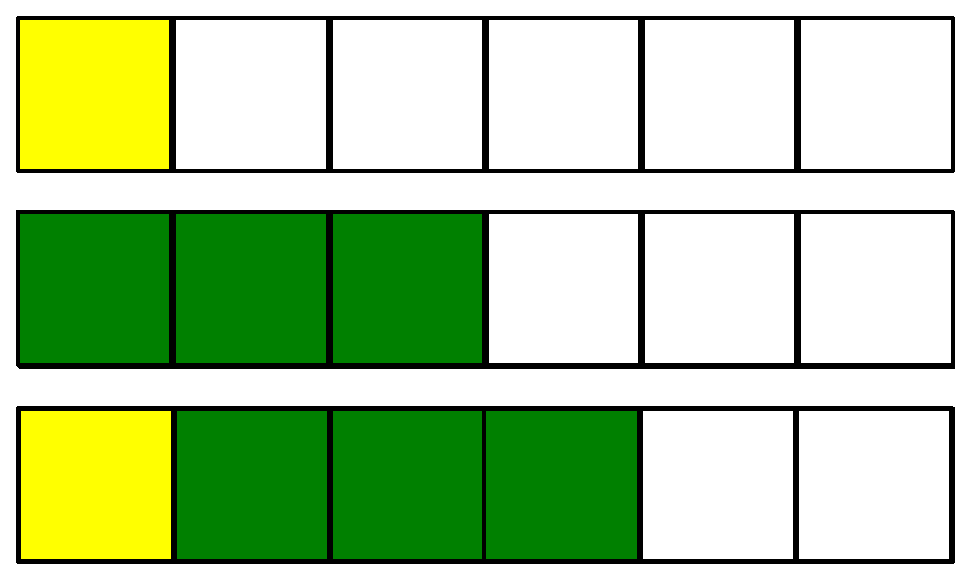
\includegraphics[height=3.5cm, width=6cm]{inicio.eps}};
	 		\draw[bole, fill = bole] (0,0) rectangle (15, -0.2);
	 		\node [right] at (7, 3.75) {{\LARGE $\frac{1}{6}$}};
	 		\node [right] at (7, 2.5) {{\LARGE $\frac{3}{6}$}};
	 		\node [right] at (7, 1.25) {{\LARGE $\frac{1}{6}+\frac{3}{6}=\frac{4}{6}$}};
	 		\end{tikzpicture}
	 	\end{figure}	 	
	 	Podemos ver que sólo sumanos los números que están en los numeradores y se mantiene el denominador en el resultado de la suma.
	 \end{itemize}
	 
	 Por lo que podemos completar el espacio en blanco de forma correcta, de la siguiente manera:
	 
	 \begin{tcolorbox}[opteqC]
	 	\def\blank#1{$\underline{\mbox{#1}}$}
	 	\begin{enumerate}%
	 		\item Pensar con el compañero de al lado hallar la forma correcta completar la oración y justifiquen su respuesta
	 		\begin{center}
	 			``\textit{Supongammos que tengo la fracción $\frac{1}{6}$ y le sumamos $\frac{3}{6}$. Entonces, se tiene un total de \blank{$\frac{1}{6} + \frac{3}{6}= \frac{4}{6}$}}''.
	 		\end{center}
	 	\end{enumerate}%
	 \end{tcolorbox}	
	\end{endmatter}
\end{document}